\documentclass{sig-alternate}
\usepackage{txfonts}
\usepackage{ifpdf}
\usepackage{amsmath}
\usepackage{mathrsfs}
\usepackage{amsfonts}
\usepackage{subfigure}
\usepackage{graphicx}
\usepackage{latexsym}
\usepackage{multirow}
\usepackage{microtype}
\usepackage{algorithm}
\usepackage{paralist}
\usepackage[sort]{cite}
\usepackage[pdfborder={0 0 0},plainpages,pdfpagelabels=false]{hyperref}

\setlength{\paperheight}{11in}
\setlength{\paperwidth}{8.5in}

\newtheorem{theorem}{Theorem}
\newtheorem{proposition}[theorem]{Proposition}
\newtheorem{claim}[theorem]{Claim}
\newtheorem{lem}[theorem]{Lemma}
\newtheorem{terminology}[theorem]{Terminology}
\newtheorem{corollary}[theorem]{Corollary}
\newtheorem{observation}[theorem]{Observation}
\newtheorem{problem}[theorem]{Problem}


\newtheorem{defi}[theorem]{Definition}
\newtheorem{exa}[theorem]{Example}

% QED symbol at the end of definitions and examples
\newif\ifqedwritten
\newenvironment{definition}[1][]{\begin{defi}[#1]\upshape\qedwrittenfalse}{\qedhere\end{defi}}
\newenvironment{example}{\begin{exa}\upshape\qedwrittenfalse}{\qedhere\end{exa}}
\newcommand{\qedhere}{\ifqedwritten\else\ifmmode\tag*{\qed}\else\hfill\qed\fi\global\qedwrittentrue\fi}

\newcommand{\topk}{\mbox{top-$k$}}
\newcommand{\Topk}{\mbox{Top-$k$}}
\newcommand{\topkm}{\mbox{top-$k$,$m$}}
\newcommand{\Topkm}{\mbox{Top-$k$,$m$}}

\renewcommand{\leq}{\leqslant}
\renewcommand{\geq}{\geqslant}

% More tolerant setting for floats -- more compactness
\renewcommand\floatpagefraction{.9}
\renewcommand\topfraction{.9}
\renewcommand\bottomfraction{.9}
\renewcommand\textfraction{.1}
\setcounter{totalnumber}{50}
\setcounter{topnumber}{50}
\setcounter{bottomnumber}{50}

\renewcommand{\textfloatsep}{1em}
\renewcommand{\dbltextfloatsep}{1em}

%%%%%%%%%%%%%%%  Magic for tighter spacing around theorem-like environments
\makeatletter
\def\@begintheorem#1#2{%
    \vspace{-3pt}
    \parskip -1pt
    \trivlist
    \item[%
        \hskip 10\p@
        \hskip \labelsep
        {{\sc #1}\hskip 5\p@\relax#2.}%
    ]
    \it
}
\let\old@endtheorem\@endtheorem
\def\@endtheorem{\old@endtheorem\vspace{-8pt}}
\makeatother

\begin{document}

%\conferenceinfo{SIGMOD '12,} {May 20--24, 2012, Scottsdale, Arizona, USA.}
%\CopyrightYear{2012}
%\crdata{978-1-4503-1247-9/12/05}
%\clubpenalty=10000
%\widowpenalty = 10000


\title{Exact and Approximate String Joins with Taxonomy}

%\numberofauthors{5}

\author{
%\alignauthor{Jiaheng Lu  \\
%       \affaddr{$^{\dag}$ School of Information and DEKE, MOE, Renmin
%University of China; Beijing, China}\\
%       \email{\{jiahenglu\}@ruc.edu.cn,  pierre@senellart.com}
%}
}


%For example, in XML keyword query refinement, each
%keyword is associated with a set of alternative terms.  Each term is
%associated with an inverted list containing the occurrences and the
%weights of the corresponding elements in the XML database. The
%\topkm{} queries return top-$k$ refined keyword combinations
%according to the corresponding \mbox{top-$m$} search results of keyword
%queries. In general, \topkm{} queries are useful in scenarios
%where the problem of selecting \emph{combinations
%of attributes} associated with ranked inverted lists naturally occurs.
%Applications range


\maketitle

\begin{abstract}

String join is an important operation in databases, data integration
and data cleansing that finds string pairs from
two collections of strings according to join predicates. This paper investigates a novel challenge to integrate taxonomy information into string joins. In particular, it presents a general-purpose strategy to improve the accuracy of string joins by enriching data with semantics-based knowledge provided by a
taxonomy (i.e., a set of is-a hierarchies) built over data items. 


We propose efficient algorithms to answer similarity join queries with taxonomy.

The extensive performance evaluation shows that the exact and approximate string joins utilize the taxonomy to improve the effectiveness of joins  and scales very well when important parameters like  data size, and number of dimensions increase.


\end{abstract}

%\category{H.2.4}{Database Management}{Systems}[Query processing]
%\category{H.3.3}{Database Management}{Information Search and
%Retrieval}[Search process]

%\terms{Algorithms, Experimentation, Performance, Theory}

%\keywords{keyword search, package search, top-$k$ querying}


\section{Introduction}



\begin{figure}[t]
\centering
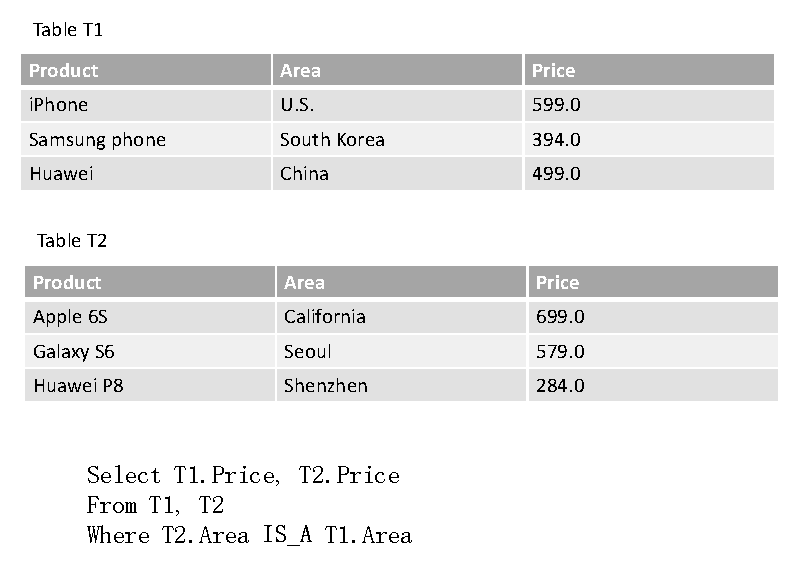
\includegraphics[width=0.45\textwidth]{figures/productexample}
 \caption{Examples to illustrate approximate joins}
\label{fig:autocompletion}
\end{figure}


Strings form a fundamental data type in computer systems and string searching has been extensively studied since the
inception of computer science. String similarity search takes a set of strings and a query string as input, and outputs all
the strings in the set that are similar to the query string. A join extends the notion of similarity search further and require
all similar string pairs between two input string sets to be reported. Both similarity search and similarity join are
central to many applications such as data integration and cleaning. 

 Taxonomies are sets of is-a hierarchies, which allow aggregating low level data items into higher level concepts. For instance, they found application in (i) mining recurrent high level associations among data as well as their temporal changes [9], [10], [11] and [12], (ii) discovering flipping correlations, i.e., patterns whose correlation flips positive to negative (or vice versa) when generalizing data items at higher abstraction levels [13], and (iii) performing social data disambiguation and analysis [14], [15], [16] and [17]. However, to the best of our knowledge, the integration of taxonomy information in data used for classifier training has never been investigated so far.




Given two strings, $s_1$ and $s_2$, we return three possible relationships between $s_1$ and $s_2$: hypernym, hyponym, mixed. For example, ``California, U.S.'' is a hyponym of ``U.S.'', ``Egypt'' is the same as ``Egypt, Africa Northern'' and ``Egypt'' is a hypernym of ``Africa''. For more examples: ``Egypt, Algeria'' is a hyponym of ``Africa Northern''.

There are two related problems: string join with taxonomy and string similarity join with taxonomy

The leave behind two intriguing questions:

1. How to efficient process string joins with taxonomy? And for multiple joins.


2. How to process the similarity joins and multiple-way similarity joins?  This question becomes increasingly urgent nowadays with the arrival of big data.

%\begin{problem}(String measure with taxonomy). Given two strings $s_1$ and $s_2$ and a taxonomy $T$, how to measure the similarity between $s_1$ and $s_2$ based on T?
%\end{problem}
%\begin{problem}(String joins with taxonomy). Given a string $p$$\in$
%$\Sigma^*$, an integer k, and a synonym set $\mathbb{R}$,  .
%\end{problem}




\subsection{Novelty and contributions}


\smallskip


Our contributions are as follows.

\noindent \textbf{Introduction of string joins with taxonomy}. We introduce a new problem to utilize the taxonomy for the string joins in databases, which has application in data integration and data cleansing.

\noindent \textbf{Holistic algorithms for multiple-way string joins} We introduce a holistic algorithm for multiple string joins.

\noindent \textbf{Introduction of approximate string joins with taxonomy}: Provide three relationships Hyper, Hypo and mixed similarity.

\noindent \textbf{Novel algorithms for multiple-way approximate string joins}


Finally, we perform experiments to evaluate our results and show the benefits of proposal algorithms.


\smallskip

The rest of this paper is organized as follows. Section 2
provides the necessary definitions, formulates . Section
3 includes our solution to JRA. In Section 4, we study
the general case of WGRAP, by reviewing the greedy algorithm
of [22], proposing our solution, analyzing its approximation
ratio, and presenting our similarity join algorithms.
Our experiments are presented in Section 5. Finally,
Section 6 concludes with a discussion about future work.


\section{Related work} \label{sec:relatedwork}

Techniques introduced in this work take a taxonomy in the
input to optimize the index structure and to process taxonomy
queries. Such a taxonomy could be constructed manually
through experts and community efforts, as in WordNet
[4], Cyc [14], and Freebase. With the advantage of freshness
and informativeness, automatic taxonomy construction has
been extensively studied recently, for example, in [20, 22,
18, 21, 26]. WikiTaxonomy [18] and YAGO [22] may be the
most notable efforts, which attempt to derive a taxonomy
from Wikipedia categories. With more web data, Probase
[26] aims at building a unified taxonomy of worldly facts.

There is a vast literature on ranked retrieval, both in the
classical and succinct settings. We report here the results
closest to our work.


 The contributions of this paper \cite{journals/vldb/MartinenghiT14}   are the following: a simple but solid framework for embedding taxonomies
into relational databases. A simple but powerful algebraic language for supporting
query relaxation: This language makes it possible to formulate, in a procedural way, complex searches over vague schemas in different application domains; a declarative, logic-based language for supporting query
relaxation: This language provides a basis for an extension
of SQL able to exploit taxonomies for expressing relaxed
queries over relational data;



Several types of Similarity Join have been proposed in the
literature, e.g., distance range join (retrieves all pairs whose distances
are smaller than a predefined threshold $\varepsilon$) [2, 3, 4, 5, 6,
7], k-Distance join (retrieves the k most-similar pairs) [8], and
kNN-join (retrieves, for each tuple in one table, the k nearest neighbors
in another table) [9, 10, 11]. The distance range join
has been one of the most studied and useful types of Similarity
Join. This type of join is commonly referred to simply as Similarity
Join and is the focus of this paper. Among its most relevant
implementation techniques, we find approaches that rely
on the use of pre-built indices, e.g., eD-index [3], D-index [4],
and List of Twin Clusters (LTC) [12]. These techniques strive
to partition the data while clustering together the similar objects.
While these indexing techniques support the SJ operation
they also have some shortcomings: D-index and eD-index may
require rebuilding the index to support queries with different $\varepsilon$,

Approximate string matching includes finding (sub)strings
that resemble a given query string. It is a well-researched
topic and has many applications, such as data cleansing [1],
spelling correction [19], query autocompletion [33], near duplicate
detection [25, 32], approximate named entity recognition
[29], and bioinformatics [20, 27, 35].
Due to the sheer amount of literature in this area, we will
focus on most related recent results and refer readers to the
excellent surveys [13, 22] and tutorials [3, 12, 16] for a comprehensive
treatment of the topic.
Based on the types of the queries, recent work focuses either
on efficient single query processing (typically named string
similarity queries) [1, 6, 9, 11, 18, 25, 28, 31], or the similarity
join which can be treated as processing a batch of similarity
queries [2, 8, 10, 12, 14, 17, 28, 29, 34, 35]. Most recently,
Jiang et al. [15] experimentally evaluate and analyze many of
the existing similarity join algorithms.



\section{Preliminaries} \label{sec:preliminaries}



In this section, we first  define taxonomy, including
hypernym and hyponym. Subsequently,
we discuss challenges of processing taxonomy-based approximate string joins.


\subsection{Taxonomy}

A taxonomy (T ,$\sqsubseteq$ ) consists of a universe of terms T and
a term-term hypernym-hyponym relationship $\sqsubseteq$.

Hypernym-hyponym relationship. The hypernym-hyponym relationship
$\sqsubseteq$ is a partial order T . For two terms t1 and t2,
we write t1 $\sqsubseteq$ t2 or t2 $\sqsupseteq$ t1, if t1 is a hypernym of t2 (or t2
is a hyponym of t1). For example, ``Caribbean Region'' is a hyponym of
``Americas''. Figure  \ref{fig:taxonomy} shows an example of taxonomy for geological locations.



Hyponymy shows the relationship between the more general terms (hypernyms) and the more specific instances of it (hyponyms). A hyponym is a word or phrase whose semantic field is more specific than its hypernym. The semantic field of a hypernym, also known as a superordinate, is broader than that of a hyponym. An approach to the relationship between hyponyms and hypernyms is to view a hypernym as consisting of hyponyms. This, however, becomes more difficult with abstract words such as imagine, understand and knowledge. While hyponyms are typically used to refer to nouns, it can also be used on other parts of speech. Like nouns, hyponyms in verbs are words that refer to a broad category of actions. For example, verbs such as stare, gaze, view and peer can also be considered hyponyms of the verb look.
Hypernyms and hyponyms are asymmetric. Hyponymy can be tested by substituting X and Y in the sentence ``X is a kind of Y'' and determining if it makes sense.[4] For example, ``A screwdriver is a kind of tool''  makes sense but not ``A tool is a kind of screwdriver''.


Hyponymy is a transitive relation, if X is a hyponym of Y, and Y is a hyponym of Z, then X is a hyponym of Z.[5] For example, violet is a hyponym of purple and purple is a hyponym of color; therefore violet is a hyponym of color. In addition, it should be noted that a word can be both a hypernym and a hyponym: for example purple is a hyponym of colour but itself is a hypernym of the broad spectrum of shades of purple between the range of crimson and violet.

The hierarchical structure of semantic fields can be mostly seen in hyponymy. They could be observed from top to bottom, where the higher level is more general and the lower level is more specific. For example, living things will be the highest level followed by plants and animals, and the lowest level may comprise dog, cat and wolf.

Under the relations of hyponymy and incompatibility, taxonomic hierarchical structures too can be formed. It consists of two relations; the first one being exemplified in 'An X is a Y' (simple hyponymy) while the second relation is 'An X is a kind/type of Y'. The second relation is said to be more discriminating and can be classified more specifically under the concept of taxonomy.

Computer science often terms this relationship an ``is-a'' relationship. For example, the phrase ``Red is-a colour'' can be used to describe the hyponymic relationship between red and colour.

Hyponymy is the most frequently encoded relation among synsets used in lexical databases such as WordNet. These semantic relations can also be used to compare semantic similarity by judging the distance between two synsets and to analyse Anaphora.

As a hypernym can be understood as a more general word than its hyponym, the relation is used in semantic compression by generalization to reduce a level of specialization.

\begin{figure}[t]
\centering
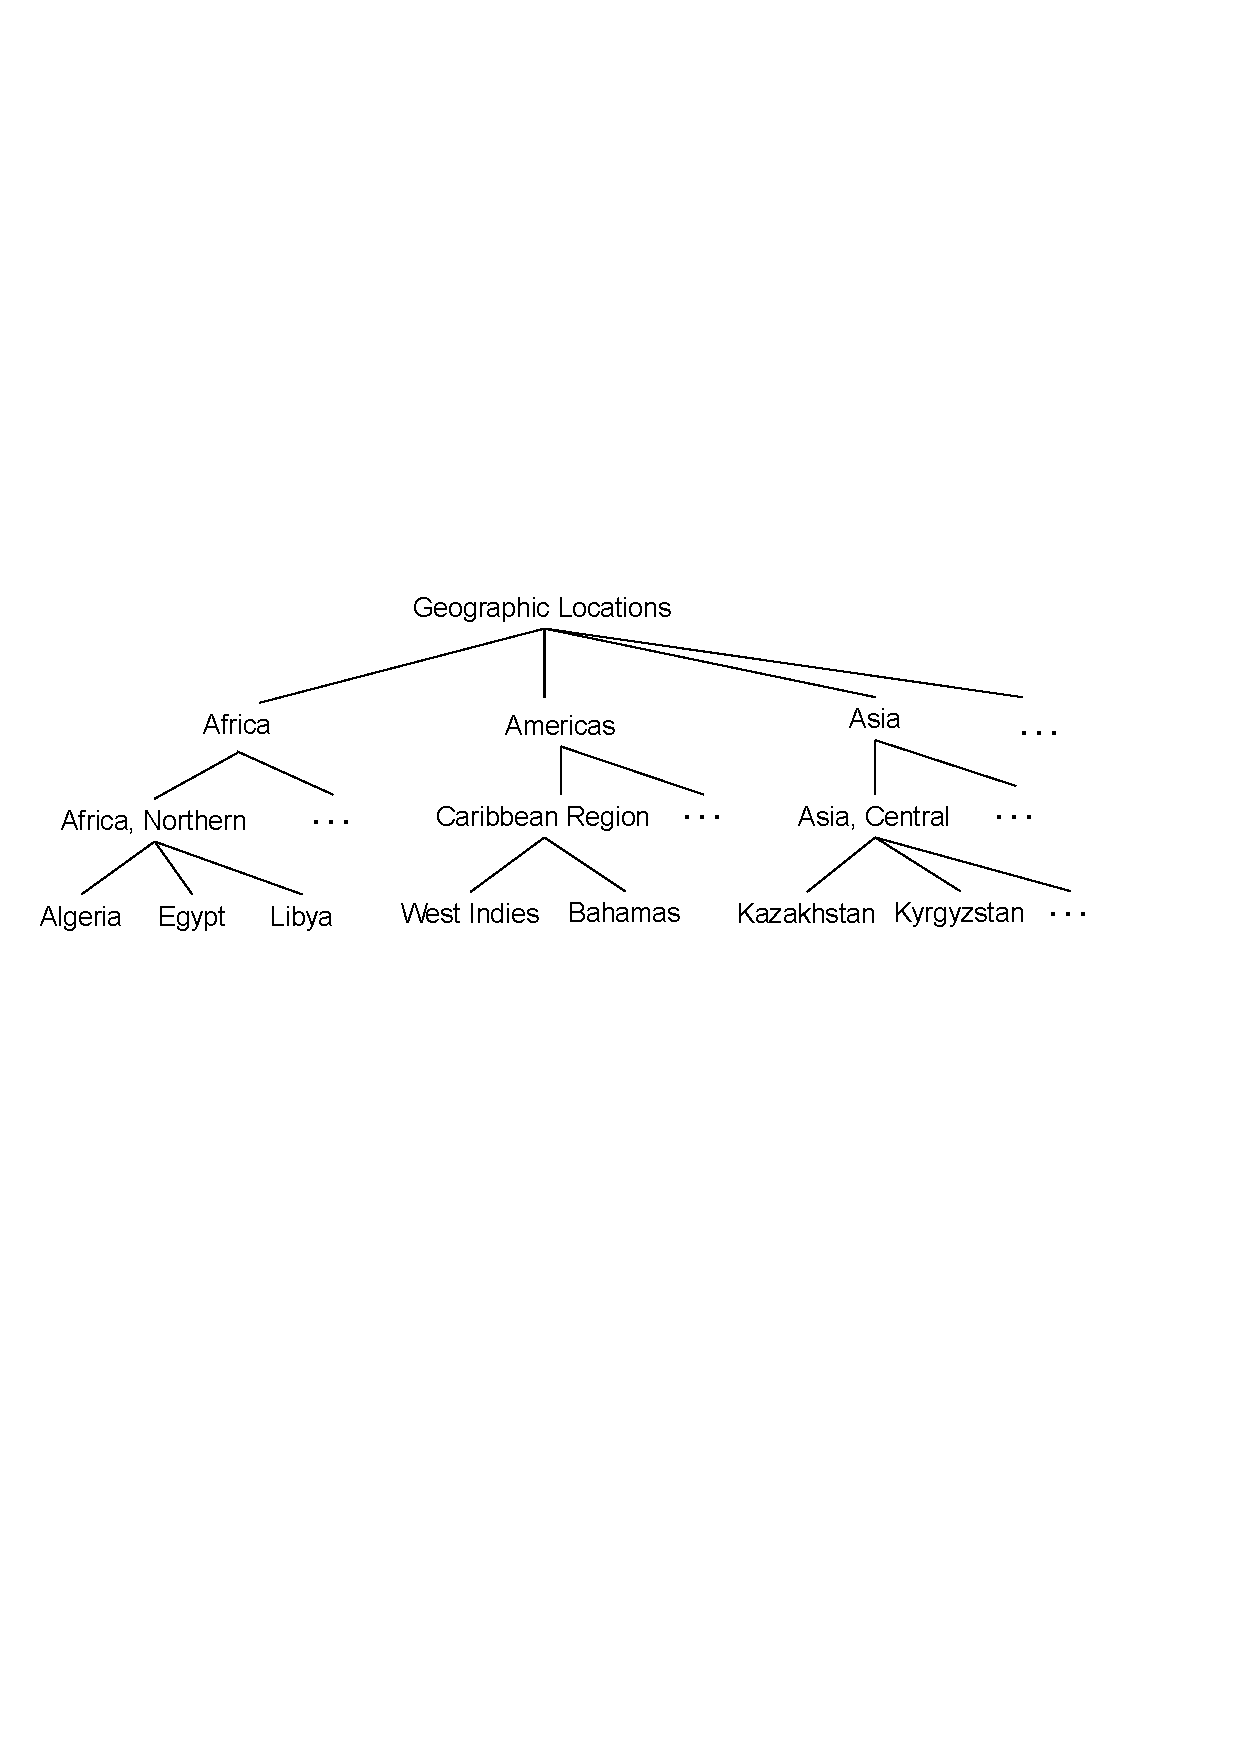
\includegraphics[width=0.45\textwidth]{figures/taxonomy}
 \caption{An example of taxonomy on ``\textsf{Geographic locations}''}
\label{fig:taxonomy}
\end{figure}

Example extended SQL

Select  T1.price, T2.price \\
From Table T1 and T2 \\
Where T1.area is\_a\_hypernym T2.area \\
With taxonomy T \\


The second SQL query:

Select  T1.price, T2.price, T3.price \\
From Table T1, T2, T3 \\
Where T1.area is\_a\_hypernym T2.area AND T1.product is\_a\_hypernym T2.product



\section{String joins with taxonomy}

We consider the exact joins including hypernymy and hyponymy and mixed three predicates based on taxonomy T.

Assume that T can fit in the main memory, this join can be implemented.

The baseline join algorithm is the nested-loop join. All string pairs are accessed to determine the hyper-hypo relationships. But this algorithm is obviously not efficient. Therefore, we propose an efficient algorithm.


Indexed base join. New indexing methods?

Label the documents, and perform the joins.

\begin{figure}[t]
\centering
\includegraphics[width=0.45\textwidth]{figures/taxonomylabels}
 \caption{An example of taxonomy with labels}
\label{fig:taxonomy}
\end{figure}



\begin{figure}[t]
\centering
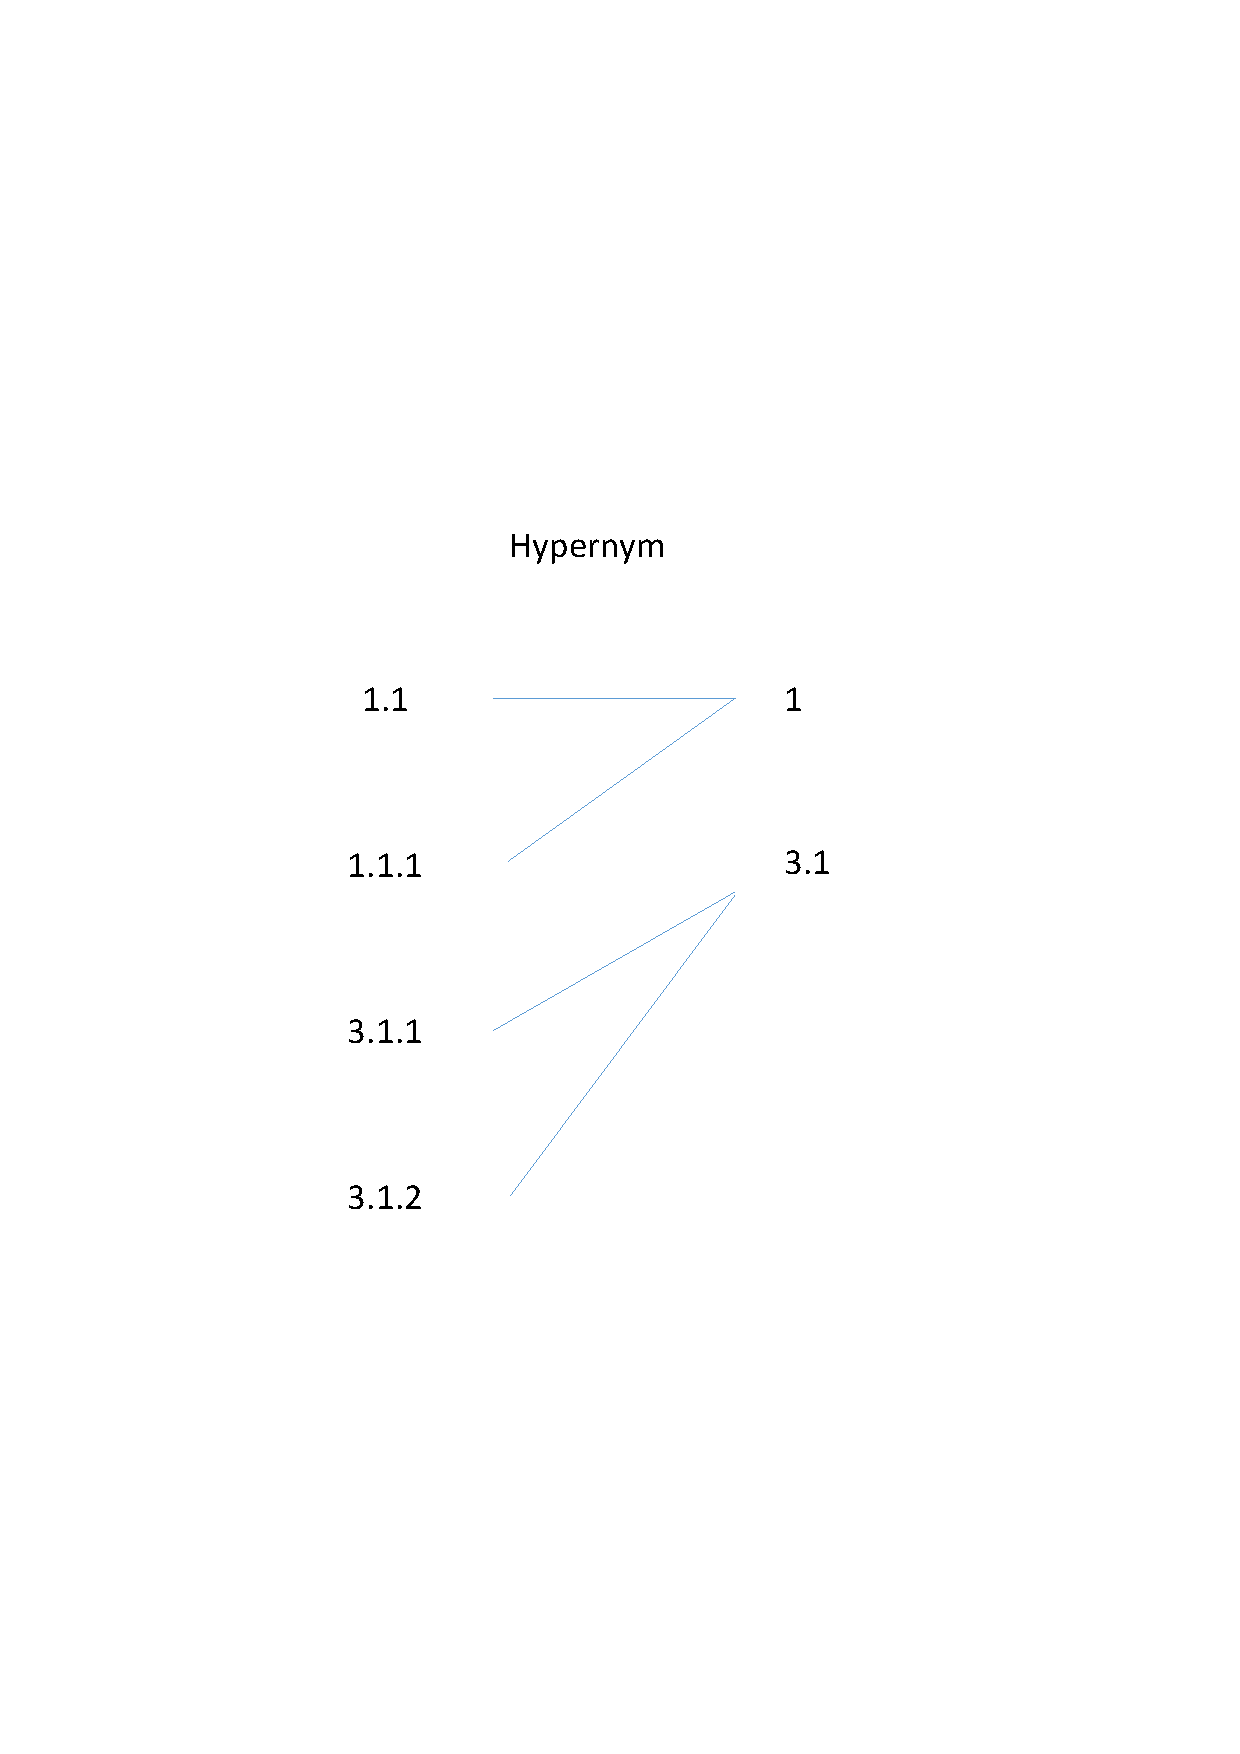
\includegraphics[scale=0.4]{figures/labeljoins}
 \caption{An example of taxonomy with labels}
\label{fig:taxonomy}
\end{figure}


%\begin{algorithm}
%{\bf Input}: two strings $s_1$ and $s_2$ \\
%{\bf Output}: four relationships: R=\{Hype, Hypo, Equa and Non\}
%\begin{compactenum}[(1)]
%\item {\bf If} ($s_1 = s_2$ )  {\bf return} Equa;
%\item {\bf If} ($|LCD(s_1)| >$ 1 AND $|LCD(s_2)| >$ 1 )  {\bf return} None;
%\item {\bf Else} {\bf if} ($|LCD(s_1)| =$ 1 AND $|LCD(s_2)| >$ 1 )
%\item \verb"  " {\bf If}  $\forall t \in LCD(s_1)$, $t$ is a hypernym of $LCD(s_2)$
%\item \verb"    " {\bf return} Hype {\bf else} {\bf return} None;
%\item {\bf Else} {\bf if} ($|LCD(s_2)| =$ 1 AND $|LCD(s_1)| >$ 1 )
%\item \verb"  " {\bf If}  $\forall t \in LCD(s_2)$, $t$ is a hypernym of $LCD(s_1)$
%\item  \verb"    " {\bf return} Hypo {\bf else} {\bf return} None;
%\item {\bf Else} /\ *  $|LCD(s_1)| = |LCD(s_2)| = $ 1 */\
%\item  \verb"  " {\bf If}  $LCD(s_1)$ is a hypernym of $LCD(s_2)$  {\bf return} Hype
%\item   \verb"  " {\bf Else if}  $LCD(s_1)$ is a hyponym of $LCD(s_2)$  {\bf return} Hypo
%\item   \verb"  " {\bf Else return} none
%\end{compactenum}
%\caption{Determine the relationship between two strings}
%\label{alg:measure}
%\end{algorithm}

\subsection{Taxonomy graph pattern}

\begin{figure}[t]
\centering
\includegraphics[scale=0.5]{figures/tgsql}
 \caption{Taxonomy graph example }
\label{fig:taxonomy}
\end{figure}

There are two kinds of edges in a graph pattern, ``$\rightarrow$'' and ``$\leftarrow$''shows the IS-A relationship, hypernym and hyponym and ``$\leftrightarrows$'' is a mixedISA relationship.

In general, at each node in the query graph pattern, there is
a node predicate on the attributes (e.g., tag, content) of the
node in question. For the purposes of this paper, exactly
what is permitted in this predicate is not material.  It suffices
for our purposes that there be efficient access mechanisms
(such as index structures) to identify the nodes in the
database that satisfy any given node predicate $q$, and
return a stream of matches $T_q$ based on the taxonomy.


Given a taxonomy graph pattern Q and an taxonomy database D, a
match of Q in D is identified by a mapping from nodes in Q
to nodes in D, such that: (i) query node predicates are satisfied
by the corresponding database nodes, and (ii) the structural (hypernym, hyponym and
mixed) relationships between query nodes are
satisfied by the corresponding database nodes. The answer
to query Q with n nodes can be represented as an n-ary relation
where each tuple ($d_1$,..., $d_n$) consists of the database
nodes that identify a distinct match of Q in D.

Given the results from taxonomy graph pattern matching, we can perform a Cartesian product to get the final results for the string joins.

\subsection{Pattern matching algorithms}

\subsubsection{Representation of nodes in taxonomy databases}

The key to an efficient, uniform mechanism for set-at-atime
(join-based) matching of query graph patterns is a positional
representation of occurrences of  elements and in the taxonomy database (see, e.g., [6, 7, 27]),
which extends the classic inverted index data structure in information retrieval [22]. We borrow the labeling scheme from XML databases and use the prefix based labels. Structural relationships between tree nodes whose positions
are recorded in this fashion can be determined easily for hypernym or hyponym relationships.

\subsubsection{Notations}

Let q (with or without subscripts) denote graph patterns.
In our algorithms, we make use of the following twig node
operations: isLeaf: Node $\rightarrow$ boolean , isRoot: Node $\rightarrow$  boolean,
parent: Node $\rightarrow$ Node, children: Node $\rightarrow$ \{Node\}, and
subtreeNodes: Node $\rightarrow$ \{Node\}. Path queries have only
one child per node, otherwise adjacent(q) returns the set
of adjacent nodes of q.

Associated with each node $q$ in a query graph pattern there
is a list $T_q$. The stream contains the positional representations
of the database nodes that match the node predicate
at the graph pattern node q. The
nodes in the stream are sorted by their prefix label. The operations over streams are: eof, advance,
next, nextL, and nextR.

\subsubsection{TGMatch Algorithm}

Algorithm TGMatch, which computes answers to a query
graph pattern, is presented in Figure 8.

Algorithm TGMatch operates in two phases. In the first
phase (lines 1-11), some (but not all) solutions to individual
query root-to-leaf paths are computed. In the second phase
(line 12), these solutions are merge-joined to compute the
answers to the query graph pattern and then the final answers are computed with Cartesian product of record IDs.

 Before a node $h_q$ from the list $T_q$ is
pushed on its stack $S_q$, TGMatch (via its call to getNext)
ensures that: (i) node $h_q$ has a descendant hq in each
of the streams Tq, for $q_i$ $\in$ adjacent($q$), and (ii) each of
the nodes hq recursively satisfies the first property.  Thus, when the query graph pattern has only
ancestor-descendant edges, each solution to each individual
query root-to-leaf path is guaranteed to be merge-joinable
with at least one solution to each of the other root-to-leaf
paths. This ensures that no intermediate solution is larger
than the final answer to the query twig pattern.

The second merge-join phase of Algorithm TGMatch is
linear in the sum of its input (the solutions to individual
root-to-leaf paths) and output (the answer to the query graph
pattern) sizes, only when the inputs are in sorted order of the
common prefixes of the different query root-to-leaf paths.
This requires that the solutions to individual query paths
be output in root-to-leaf order as well, which necessitates
blocking; showSolutions (from Figure 5), which outputs
solutions in sorted leaf-to-root order, cannot be used.

\subsubsection{Analysis of TGMatch}

 We discuss the correctness of algorithm TGMatch for processing string joins with taxonomy, and then we analyze its complexity.

 \begin{definition}[minimal descendant extension] Consider a pattern query Q. For each node
q $\in$ scope(Q) we define the head of $q$, denoted $h_q$,
as the first element in $T_q$ that participates in a solution for
the sub-query rooted at $q$. We say that a node q has a minimal
descendant extension if there is a solution for the subquery
rooted at q composed entirely of the head elements of
subtreeNodes ($q$).
\end{definition}

\smallskip

\begin{theorem}
 Given a query graph pattern g and a taxonomy
database D, Algorithm TGMatch correctly returns all answers
for g on D.
\end{theorem}

While correctness holds for query graph patterns, we can prove
optimality. The intuition is simple.
Since we push into the stacks only elements that have both
a descendant and an ancestor extension, we are guaranteed
that no element that does not participate in any solution is
pushed into any stack. Therefore, the merge postprocessing
step is optimal, and we have the following result.


\begin{theorem}
 Consider a query graph pattern g with n
nodes, and only ancestor-descendant edges, and a taxonomy
database D. Algorithm TGMatch has worst-case I/O and
CPU time complexities linear in the sum of sizes of the
n input lists and the output list. Further, the worst-case
space complexity of Algorithm  TGMatch is the minimum
of (i) the sum of sizes of the n input lists, and (ii) n times
the maximum length of a root-to-leaf path in D.
\end{theorem}

\section{String similarity joins with taxonomy}


We extend our definition to composite relation. For example: ''U.S and China'' is a composite hyponym of ``California and Beijing''. Another example: ``Hong Kong and California'' and ``U.S.''. This is a partial hypernym relation, since only California is a hypernym of U.S.

The sort-merge algorithm cannot work here.

Labeling scheme and the join:

If there are more than one string, then we can perform the verification after the filtering.


 Therefore, we propose a labeling scheme to process. Convert it to the ancestor-descendant joins



\subsection{Similarity measures}



We define the taxonomy similarity between two strings:

\begin{definition}[Taxonomy intersection]
Given two token sets $S_1$ and $S_2$, and a taxonomy $\mathcal{T}$, we say an element (token) $e \in S_1 \bigcap_T S_2$ if one the following cases is satisfied:

(1) $ e \in S_1$ (resp. $S_2$) and $\exists t \in S_2$ (resp. $S_1$), s.t. $(e,t) \in \mathcal{T} $, or

(2) $ e \in S_1$, and $e$ is a token of $e'$, and every token $e''$ in $e$ is in the set $S_1$, s.t. $\exists (e',t) \in \mathcal{T}$.\end{definition}

\begin{definition}[Taxonomy similarity]   Given two sets of tokens $S_1$ and $S_2$,we define the taxonomy similarity (TS) between $S_1$ and $S_2$ as follows:

\begin{equation}
TS(S_1,S_2)=  \frac{(S_1 \bigcap_T S_2) \bigcup (S_1 \bigcap S_2) }{S_1 \bigcup S_2}
\end{equation} \end{definition}

\subsection{String similarity join algorithms}

\subsubsection{Graph pattern with similarity thresholds}

\begin{figure}[t]
\centering
\includegraphics[scale=0.4]{figures/tgsql2}
 \caption{Taxonomy graph example }
\label{fig:similaritygeaph}
\end{figure}

See Figure \ref{fig:similaritygeaph} for an example of similarity graph to perform similarity joins.

\textbf{Baseline algorithm}. We can use the similar algorithm as that in string exact join with taxonomy. And then use these candidate for filtering. But this baseline algorithm has one limitation that there are too many candidates. Then we show how to perform the second filtering to reduce the number of candidate pairs.

\textbf{Signature-based index}. Given a string s with length $|s|$, then the size of signature is $\lceil (1-\theta)|s| \rceil$. But if the signatures involve the taxonomy, then we cannot make this argument.

But if in some real cases, we select the word from taxonomy as signatures. Therefore we need to compute a relax maximum similarity. In this case, we still do not need to retrieve the whole string to compute real similarity.

Given as string $s$, assume that its applied taxonomy node is $n$.

In this paper, we propose a new index which combine a signature filters and a length together with a bit-matrix, which extends bloom filter to two dimensions.

In the literature, the current "modus operandi" is called \textit{prefix filter}, which is based on the intuition that if two canonicalized records are similar, some fragments of them should overlap with each other, as otherwise the two records
won't have enough overlap. This intuition can be formally captured by the prefix-filtering
principle \cite{conf/icde/ChaudhuriGK06} rephrased below.

\begin{lem} (\textsc{Prefix filter principle}) \cite{conf/icde/ChaudhuriGK06} Given an
ordering $O$ of the token universe $U$ and two strings $s$ and $t$, each with tokens sorted in the
order of $O$.   If Jaccard($s, t$) $\geq \theta$, then the first $\lceil(1-\theta)|s|\rceil$ smallest
tokens of $s$ and the first $\lceil(1-\theta)|t|\rceil$ smallest
tokens of $t$  must share at least one token.
\end{lem}

\subsubsection{Bloom matrix}

We develop a new bloom matrix to extend the bloom filtering to quickly decide if there are any possibility that two sets of collections can produce at least one matching pair.

There are three conditions

(1) There are no overlapping for non-taxonomy bloom matrixes.

(2) No taxonomy relationships and no signature bloom filter with taxonomy tokens.

(3) Length filtering for those taxonomy strings.

If (1) and (3) OR (1) and (2) are satisfied, then there are no any solution. We can quickly skip the join for those two collections. Otherwise we need to go into the collection and use the following algorithm to find the join solutions.


\subsubsection{Subset prefix filtering}

Given strings which do not contain enough non-taxonomy signature tokens, we need some special processing.

Assume that a string $s$ has $v_1$ in the taxonomy tree, then all strings which have not the taxonomy relationships with $v_1$ should have the overlapping prefix signature with $s$, therefore we can impose the prefix i=filtering again, but the number of prefix should be revisited. In addition, for string which has the taxonomy relationship with $v_1$, then we can only apply the length filtering.

%For strings which do not contain any non-taxonomy words, we propose a bipartite grouping index. The main idea is to separate the strings to several groups and for different groups, there is no need to compare the strings.
%There are also methods that exploit triangle inequality to support edit distance-based similarity queries [27]. Edit distances of every data string to pre-chosen reference strings are precomputed, and used by the query processing algorithm to filter non-promising data strings based on the triangle inequality. Several issues regarding judicious selection of reference objects are studied in [27]. Alternatively, existing metric indexes [36] can be used for query processing too. As this line of methods is applicable to any metric distance, they cannot attain ultra fast performance. But in this paper, we select multiple groups and therefore we can obtain better performance.
%Multiple reference points, and therefore we can prune away strings by those multiple reference points.



\section{Experimental analysis}

To evaluate the effectiveness of the proposed top-$k$ completion
techniques, Expansion Trie (ET), Two tries (TT), and  Realizer Trie (RT), we will compare
their effectiveness on the following datasets from different
application scenarios in Java $1.6.0$ and run on a
Windows XP with dual-core Intel Xeon CPU 4.0GHz, 2GB RAM, and a 320GB hard disk.


\subsection{Datasets}
We use three datasets: US addresses (\textbf{USPS}),
conference titles  (\textbf{CONF}), and gene/protein data
(\textbf{SPROT}). These datasets differ from each other in terms of rule-number, rule-complexity, data-size and string-length. Our goal in choosing these diverse sources is to understand the usefulness of algorithms in different real world environments.

\smallskip
\noindent \textbf{{USPS}}: We downloaded common person names, street names,
city names, states, and zip codes from the United States Postal
Service website ({\footnotesize http://www.usps.com}). We then generated
one million records, each of which contains a person name, a street
name, a city name, a state, and a zip code. USPS also publishes
extensive information about the format of US addresses, from which we
obtained 284 synonym pairs. The synonym pairs covers a wide range of alternate
representations of common strings, e.g. street $\rightarrow$ st.


\noindent \textbf{{CONF}}: We collected 10,000 conference names
from more than ten domains, including Medicine and Computer
Science.
We obtained $1000$ synonym pairs between the full names of conferences and their
abbreviations by manually examining conference websites or homepages
of scientists.


\noindent \textbf{{SPROT}}: We obtained one million gene/protein records
from the Expasy website ({\footnotesize http://www.expasy.ch/sprot}).
Each record contains an identifier (ID) and its name.
%For example, the two records, \textit{(O00203, Adapter-related protein complex 3
%beta-1 subunit)} and \textit{(O00203, AP-3 complex subunit
%beta-1)}, refer to the same gene as they have the same ID.
In this dataset, each ID has $5\sim22$ synonyms. We generated 10,000 synonym rules describing gene/protein
equivalent expressions.

In each dataset we subtracted from the scores their minimum,
so that the smallest score is 0, without affecting the
ordering. The minimum is then added back at query time.




\begin{figure}
  \small
  \centering
  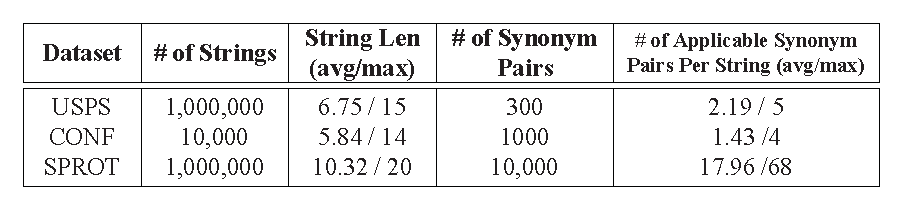
\includegraphics[width=\linewidth]{figures/Characteristics_Datasets}
   \vspace{-6mm}
  \caption{Characteristics of Datasets.}
  \label{tab:data_characteristics}
\end{figure}


Figure~\ref{tab:data_characteristics} gives the characteristics of the
three datasets.


\subsection{Space}

We evaluate the compactness of the data structures by
reporting in Table 1 the average number of bits per string
(including score). For comparison, we also report the size
of the original uncompressed text file (Raw) and the gzip
compressed binary (GZip). Across the 4 datasets, the three
presented techniques achieve an average compression ratio
of between 29\% and 51\%, with SDT consistently having the
smallest size. In fact, its size is only 3\% larger than that
achieved by gzip compression on average, and is actually
10\% smaller on the Unigrams datatset.



To better understand how the space is used, we present
in Figure 8 the storage breakdown of each of the techniques
on QueriesA. For CT, 70  the space is used to store the
uncompressed character sequences. Compressing the node
character sequences with RePair [22] can further reduce the
size, but will incur some sacrifice in speed. With delta encoding,
storing the scores, including the 2 bit header, takes
only 4.0 and 9.6 bits per node and string, respectively. In
comparison, standard variable-byte encoding with a single
continuation bit [38] requires at least 8 bits per node. Similarly,
we utilize an average of only 16.4 bits per string in the
dataset to encode the tree structure. As reference, it would
have required 24 bits just to encode the index of a string.

\subsection{Time}

To evaluate the runtime performance of the proposed data
structures, we synthesize a sequence of completion requests
to simulate an actual server workload. Specifically, we first
sample 1M queries in random order from the dataset according
to the normalized scores. Assuming that user queries
arrive according to a Poisson process, we can model the interarrival
time of each query using an exponential distribution.
We can control the average queries per second (QPS) by
adjusting the  parameter of the exponential distribution.
For simplicity, we assume that each subsequent keystroke
arrives 0.3 seconds apart, corresponding to an average typing
speed of 40 word per minutes. Users will continue to enter
additional keys until the target query appears as the top
suggestion, or until the query has been fully entered. Note
that with higher QPS, requests from different queries are
more likely to overlap, leading to more cache misses.
In Table 2, we present the mean time to compute the top-10
completions, averaged over 10 runs. Overall, CT achieves the
best performance, about twice as fast as SDT. While much
of the differences can be attributed to SDT's use of succinct
operations for trie traversal and RePair decoding of label
sequence L, CT's better memory locality, where all node
information are stored together, still plays an important
part. For instance, we see that when the nodes are not
arranged for locality, as is the case for RT, the performance
is extremely poor. Similarly, as the requests corresponding
to higher QPS exhibit less overlap in memory access, the
performance degrades by an average of 10\% for CT and 21\%
for SDT. As the prefixes used by the two workloads differ only
in order, the performance gap is due entirely to the effect
of CPU cache, where CT shines. To simulate a moderate
workload, we use 1K QPS in the remaining analyses.


To better understand the performance differences between
the techniques, we break down the total time to compute the
top-10 completions on QueriesA into the time spent finding
the locus node and computing each successive completion.
As shown in Figure 9, CT using pointer arithmetic is significantly faster than data structures using balanced parentheses
for traversal, especially in finding the initial locus node. Theoretically,
the cost of retrieving each additional completion
increases logarithmically. But in practice, the incremental
cost for both CT and SDT remains mostly constant (not
shown), as it is dominated by memory access time, with
decreasing probability of cache miss for each additional completion.
In fact, for RT, it actually takes less time to compute
each additional completion. Furthermore, although we are
also returning the completion string, each completion in SDT
is about twice as fast as a random Access operation. CT has
an even larger ratio due to its less efficient Access operation.
Thus, by integrating string construction into the completion
algorithm, we significantly reduce the overall time required to
enumerate the top-k completions.

\subsection{Scalability}

To assess the scalability of the data structures, we compare
their performance on different size subsets of the QueriesB
dataset. Specifically, to mimic practical scenarios where we
have a limited memory budget and can only accord to serve
the most popular queries, we will generate these subsets by
taking the top-N distinct queries in decreasing score order.
Figure 10 plots the change in average bytes per query as we
increase the number of queries. Overall, we see that lower
count tail queries are longer and require more space across all
techniques, likely due to the different characteristics exhibited
by queries with only a few counts. While SDT requires more
space than CT below 100 queries due to its large sublinear
overhead, its size continues to fall with increasing number of
queries and actually becomes smaller than GZip on a wide
range of dataset sizes.
We present in Figure 11 the effect the number of queries
has on the average time per completion for top-10 completion
requests. We use the synthesized workload based on the full
QueriesB dataset to best approximate real world usage scenarios
where users enter prexes without knowing what queries
the system can complete. Thus, both the average number of
completions and average completion length increase with the
dataset size. As shown, the average time per completion for
CT increases very slowly, due to increasing completion length
and more cache misses. It is higher for smaller datasets as



%***************************************Conclusion and future work************************************
\section{Conclusion and future work}

We introduce a new query type, approximate string join, with taxonomy. We propose processing
models for taxonomy queries, and introduce how to build
an additional index (besides the inverted index) to support
efficient query processing. In particular, we study the problem
of how to optimize this additional index based on a
workload of queries, with the goal of minimizing query processing
cost, and propose algorithms with performance guarantees.
Our index optimization techniques are tested using
real datasets and are shown to be effective and robust.



\bibliographystyle{abbrv}
\bibliography{localrefs}



\end{document}
